\documentclass[letterpaper,12pt,twoside,]{pinp}

%% Some pieces required from the pandoc template
\providecommand{\tightlist}{%
  \setlength{\itemsep}{0pt}\setlength{\parskip}{0pt}}

% Use the lineno option to display guide line numbers if required.
% Note that the use of elements such as single-column equations
% may affect the guide line number alignment.

\usepackage[T1]{fontenc}
\usepackage[utf8]{inputenc}

% pinp change: the geometry package layout settings need to be set here, not in pinp.cls
\geometry{layoutsize={0.95588\paperwidth,0.98864\paperheight},%
  layouthoffset=0.02206\paperwidth, layoutvoffset=0.00568\paperheight}

\definecolor{pinpblue}{HTML}{185FAF}  % imagecolorpicker on blue for new R logo
\definecolor{pnasbluetext}{RGB}{101,0,0} %


\usepackage{wrapfig,subcaption,array,tabularx,multirow,caption} \usepackage[utf8]{inputenc}

\title{QBUS2820 Assignment2}

\author[]{}


\setcounter{secnumdepth}{0}

% Please give the surname of the lead author for the running footer
\leadauthor{}

% Keywords are not mandatory, but authors are strongly encouraged to provide them. If provided, please include two to five keywords, separated by the pipe symbol, e.g:
 

\begin{abstract}

\end{abstract}

\dates{This version was compiled on \today} 

% initially we use doi so keep for backwards compatibility
% new name is doi_footer

\pinpfootercontents{QBUS2820 Assignment 1}

\begin{document}

% Optional adjustment to line up main text (after abstract) of first page with line numbers, when using both lineno and twocolumn options.
% You should only change this length when you've finalised the article contents.
\verticaladjustment{-2pt}

\maketitle
\thispagestyle{firststyle}
\ifthenelse{\boolean{shortarticle}}{\ifthenelse{\boolean{singlecolumn}}{\abscontentformatted}{\abscontent}}{}

% If your first paragraph (i.e. with the \dropcap) contains a list environment (quote, quotation, theorem, definition, enumerate, itemize...), the line after the list may have some extra indentation. If this is the case, add \parshape=0 to the end of the list environment.


\captionsetup[figure]{labelfont={it,bf,scriptsize},textfont={it,scriptsize},labelsep=colon}
\captionsetup[table]{labelfont={it,bf,scriptsize},textfont={it,scriptsize},labelsep=colon}
\captionsetup[FLOAT_TYPE]{labelformat=simple, labelsep=colon}

\hypertarget{task-a}{%
\section{Task A}\label{task-a}}

\hypertarget{introduction}{%
\section{Introduction}\label{introduction}}

In a traditional manner, sale prices of houses were predicted by
comparing sale prices and costs in the real estate market. There was no
general standard to estimate the value of houses. Machine learning
techniques therefore play an important role to help establishing models
for sale prices of house predictions. As mentioned by Calhoun, the
availability of a house price prediction model helps fill up an
essential information gap and improve the efficiency of the real estate
market (Calhoun, 2003).

This project aims to develop predictive models for sale prices of house
with machine learning techniques. With the sale price which is a
numerical variable being the response of predictive models, six models
are developed and validated.

By comparing the root mean squared errors of predictions, the lasso
regression model and random forest model are found to have the best
predictive performance for the housing data, compared to elastic net,
ridge regression, k-nearest neighbor regression and stepwise regression
with forward selection.

\hypertarget{data-processing-and-exploratory-data-analysis}{%
\section{Data processing and exploratory data
analysis}\label{data-processing-and-exploratory-data-analysis}}

There are 36 numeric variables and 43 categorical variables in the
housing data. By calculating the correlation coefficient, 12 numeric
variables are found to be potentially linearly related to sale price, as
the absolute values of corresponsing carrelation coefficients are
greater than 0.5. The distributions of these variables are visualised in
figure \ref{fig:scatter}. `TotRms AbvGrd', `Garage Area', `1st Fir SF'
and `SalePrice' are shown to be right-skewed while `Garage Yr Blt' and
`Overall Qual' are left-skewed, but these distributions are
significantly influenced by outliers in several columns. Moreover, some
variables, such as `TotRms AbvGrd', tend to have linear relationships
with other variables except sale price, leading to multi-collinearity.
This could violate the assumption of some predictive models, such as
multiple linear regression, thus robustness to multi-collinearity should
be carefully considered when developing predictive models.

Figure \ref{fig:boxplots} shows the distribution of sale price with
regard to different categorical features. For most categorical features,
sale prices tend to largely different for different groups of the
categorical feature, except `BsmtFin Type 2' and `Land Slope'. However,
although medians sale prices look similar for different groups of
`BsmtFin Type 2' and `Land Slope', the distribution of sale prices are
not identical. Hence, it can still be worthwhile to includue these two
variables as features to predict sale price. In addition, the boxplots
also highlight the ouliers of sale price existing in diifferent
categorical groups.

Besides affecting the shapes of data distribution, the existing outliers
of numeric variables can also post a significant effect on predictive
performance when making sale price predicions.Therefore data
pre-processing needs to be considered in the stage of feature
engineering in order to overcome issues caused by outliers.

\hypertarget{feature-engineering}{%
\section{Feature engineering}\label{feature-engineering}}

\begin{wrapfigure}{r}{0.5\textwidth}
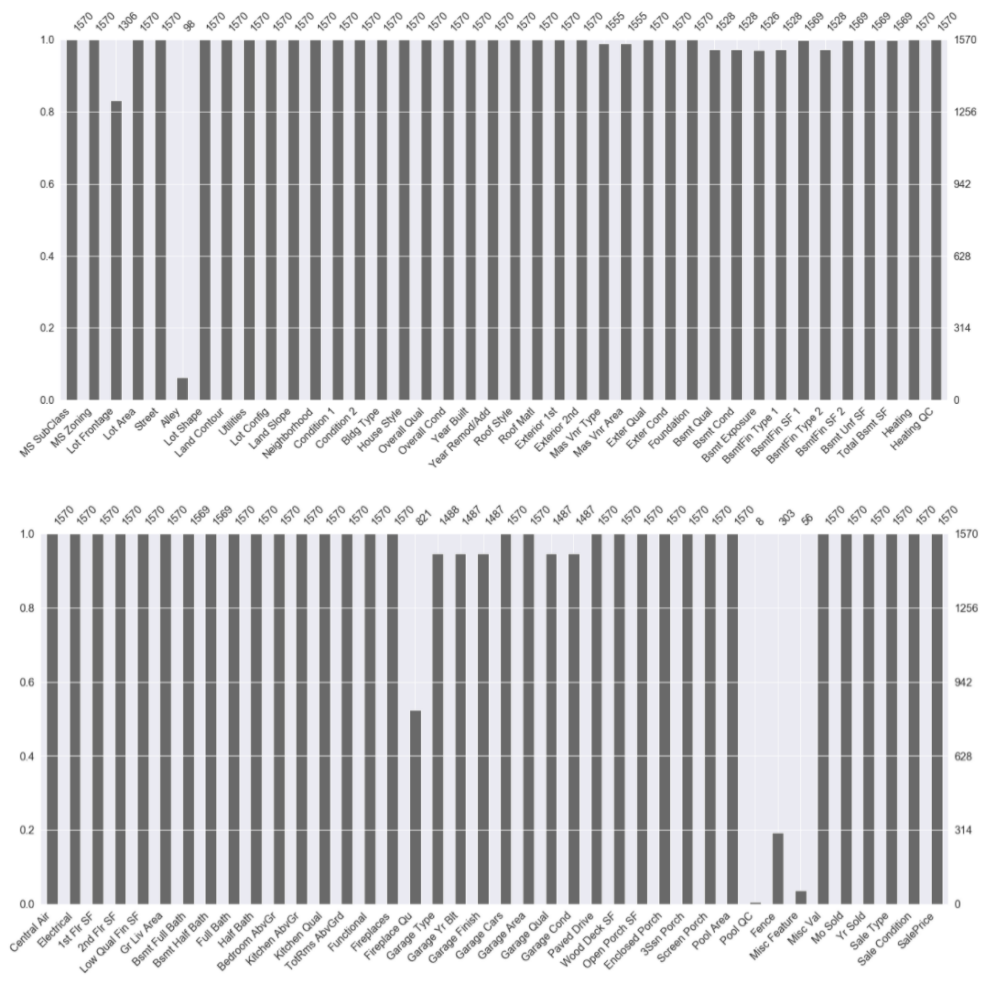
\includegraphics[width=1\linewidth]{miss_plot.png}
\centering
\caption{Visualizing missingness of housing data in training set.}
\label{fig:miss}
\end{wrapfigure}

As shown in Figure \ref{fig:miss}, there are huge amounts of missing
values in several columns: `Alley', `Fireplace Qu', `Pool QC', `Fence',
`Misc Feature', with more than 40\% missing values within each column.
With this issue, such variables are uninformative to be a feature of
predictive models as there are too few observations. To deal with this,
removing all rows with missing values can lead to significant loss of
information, while imputation using small amount of observations can
misrepresent the population for largely incomplete columns. Therefore,
`Alley', `Pool QC', `Fence', `Misc Feature' are abandoned due to high
missing rates.

Besides, there are 19 columns containing missing values but the
percentages of missing values are less than 20\%. This can be deal with
by imputation. The missing values are imputed by using the most frequent
value of each column.

As mentioned before, outliers exist with most of numeric features, which
could be a big concern for predictive performance. Data standardization
is therefore performed for numeric variables by subtracting the mean,
followed by dividing the standard deviation of the corresponding
columns.

After feature engineering, there are 74 informative features, with 36
features being numeric and 38 features being categorical. There are 1570
observations in the training set and 1210 observations in the testing
set. For regression models involving categorical features, dummy
variables are created for each categorical feature.

\hypertarget{methodology}{%
\section{Methodology}\label{methodology}}

Five regression models are trained by two sets of data where one
training set contains numeric features only and the other set includes
both categorical and numeric features. With regards to the issue of
multi-collinearity mentioned before, all of the five regression
techniques used are capable for addressing multi-collinearity. As such,
the features surviving in feature engineering are all fed into
predictive models.

To develope the best parameter set for each regression models,
hyperparameters of are tunned with 5-fold cross validation. The
performance of models with different value of hyperparameters is
estimated by negative mean squared error, where a larger score indicates
better predictive performance.

\hypertarget{random-forest-regression}{%
\subsection{Random forest regression}\label{random-forest-regression}}

Random Forest uses bootstrap sampling and feature sampling, i.e row
sampling and column sampling. Therefore Random Forest is not affected by
multicollinearity that much since it is picking different set of
features for different models and of course every model sees a different
set of data points.

This tells us the most important settings are the number of trees in the
forest (n\_estimators) and the number of features considered for
splitting at each leaf node (max\_features).

\hypertarget{lasso-regression}{%
\subsection{Lasso Regression}\label{lasso-regression}}

Least absolute shrinkage and selection operator (Lasso), as an extension
of liner regression analysis, conducts both feature selection and
regularization. This helps to enhance the predictive performance and
interpretability of the model developed.

The objective of a lasso regression model is to minimize
\(\sum^n_{i=1}(y_i-\sum_jx_{ij}\beta_j)^2+\alpha\sum^p_{j=1}|\beta_j|\),
where \(\alpha\) is a tuning parameter which represents how strong the
L1 regularization penalize coefficients of the lasso regression model.
Changing the value of \(\alpha\) influences the number of features
eliminated. When \(\alpha=0\), coefficients of features are not
Palisades such that no feature is removed. As the value of \(\alpha\)
increases, L1 penalty gets stronger and therefore more features are
eliminated, vice versa. Furthermore, the value of \(\alpha\) also
affects the bias-variance trade-off. An increase of \(\alpha\) leads to
increase in bias while a decrease of \(\alpha\) results in increase in
variance.

\hypertarget{ridge-regression}{%
\subsection{Ridge Regression}\label{ridge-regression}}

Ridge Regression is a technique for analyzing multiple regression data
that suffer from multicollinearity. When multicollinearity occurs, least
squares estimates are unbiased, but their variances are large so they
may be far from the true value.

can do certain level of feature selection

\hypertarget{elastic-nets}{%
\subsection{Elastic Nets}\label{elastic-nets}}

Several researchers and data scientists have worked hard to explore the
value of procedures like ElasticNets to help resolve the L1/L2 debate to
multicollinearity correction. Through this technique, we are able to
combine the strengths of both Ridge and LASSO regression, while
minimizing the negative impact of either of these procedures. Some
advantages of Elastic Net is that it is able to (1) enforce sparsity,
(2) it has no limitation on the number of selected variables, and (3) it
encourages a grouping effect in the presence of highly correlated
predictors. A main disadvantage of this technique is that a naïve
elastic net can suffer from double shrinkage, therefore, one needs to be
careful when employing this option. If a naïve elastic net is found, a
correction does exist to help control for this

\hypertarget{stepwise-regression-with-forward-selection}{%
\subsection{Stepwise regression with Forward
Selection}\label{stepwise-regression-with-forward-selection}}

\begin{wraptable}{r}{8cm}
\begin{tabular}{ |c|c|c| } 
\hline
\textbf{Model / Features} & \textbf{Numeric} & \textbf{Numeric and Categorical} \\
\hline
\textbf{Forward selection} & 34470.77 & $5.21\times 10^{15}$ \\ 
\textbf{Lasso} & 34543.61 & 29628.07 \\
\textbf{Ridge} & 34475.68 & 30082.79 \\
\textbf{Elastic net} & 35380.58 & 32844.26 \\
\textbf{Random forest} & 28016.33 & 28805.04\\
\hline
\end{tabular}
\centering
\caption{Summary of predictive performance for regression models. The performance measurement metric is the root mean squared error from cross validation.}
\label{table:cv_errors}
\end{wraptable}

\hypertarget{validation-set-results}{%
\section{Validation set results}\label{validation-set-results}}

\hypertarget{conclusion}{%
\section{Conclusion}\label{conclusion}}

\hypertarget{references}{%
\section{References}\label{references}}

\begin{itemize}
\tightlist
\item
  Gibson, M., Little, R. and Rubin, D., 1989. Statistical Analysis with
  Missing Data. The Statistician, 38(1), p.82.
\item
  Scikit-learn.org. 2020. 6.4. Imputation Of Missing Values ---
  Scikit-Learn 0.23.2 Documentation. {[}online{]} Available at:
  \url{https://scikit-learn.org/stable/modules/impute.html}.
\item
  Scikit-learn.org. 2020. 6.4. Imputation Of Missing Values ---
  Scikit-Learn 0.23.2 Documentation. {[}online{]} Available at:
  \url{https://scikit-learn.org/stable/modules/impute.html}.
\item
  Hintze, J.L., 1992. Chapter 335: Ridge Regression. In Number cruncher
  statistical system: statistical software. Kaysville, UT: Jerry L.
  Hintze.
\item
  Chakon, O. (2017). Practical Machine Learning: Ridge Regression Vs
  Lasso. Coding Startups: Coders With Entrepreneurial Mindset. Published
  August 3rd, 2017.
\item
  Allison, P. (2012). When Can You Safely Ignore Multicollinearity?
  Statistical Horizons.
\item
  Cross Validated. (2015). What is elastic net regularization, and how
  does it solve the drawbacks of Ridge (L2) and Lasso (L1)? {[}online{]}
  Available at:
  \url{https://stats.stackexchange.com/questions/184029/what-is-elastic-net-regularization-and-how-doesitsolve-the-drawbacks-of-ridge/184031\#184031}.
\end{itemize}

\hypertarget{task-b}{%
\section{Task B}\label{task-b}}

\hypertarget{exploratory-data-analysis}{%
\section{Exploratory data analysis}\label{exploratory-data-analysis}}

\begin{wrapfigure}{r}{0.5\textwidth}
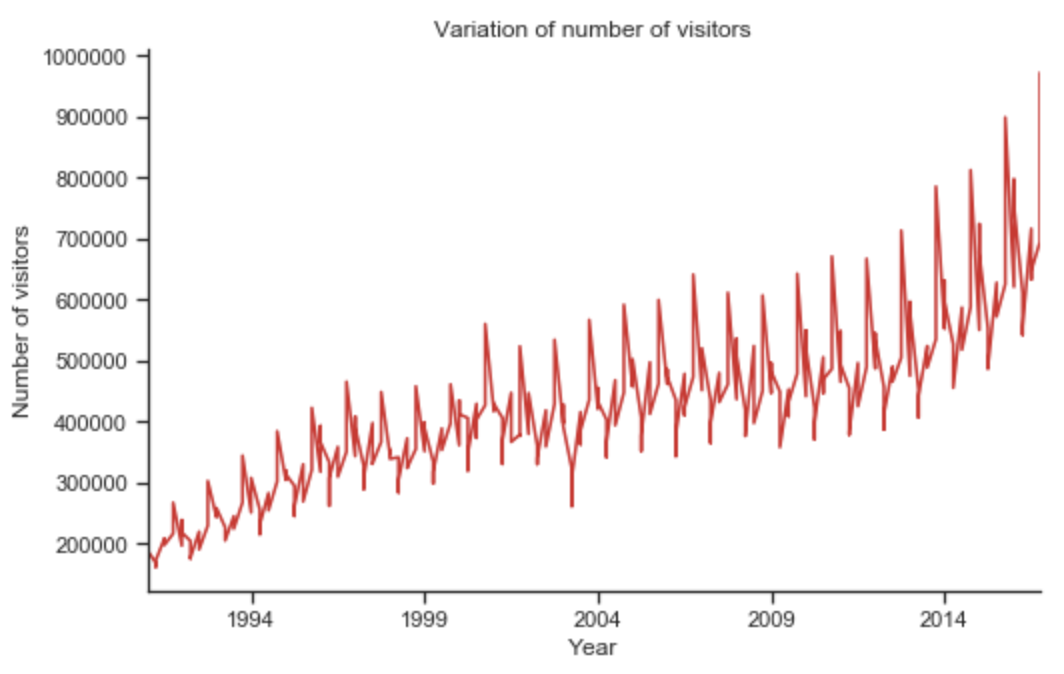
\includegraphics[width=1\linewidth]{timeseries.png}
\centering
\caption{Time series of number of visitors from 1991 to 2016.}
\label{fig:timeseries}
\end{wrapfigure}

The time series plot figure \ref{fig:timeseries} shows an upward trend
from 1991 to 2016, with a seasonal pattern as symtematic changes occur
in short periods which are fixed. Furthermore, the variation of number
of visitors within the fixed period becomes greater as time moves. As
such, a multiplicative forecasting model may be more suitable for this
data compared to an additive model.

\hypertarget{forecasting-models}{%
\section{Forecasting models}\label{forecasting-models}}

\hypertarget{seasonal-random-walk}{%
\subsection{Seasonal random walk}\label{seasonal-random-walk}}

\hypertarget{drift-model}{%
\subsection{Drift model}\label{drift-model}}

\hypertarget{exponential-smoothing}{%
\subsection{Exponential smoothing}\label{exponential-smoothing}}

\hypertarget{appendix}{%
\section{Appendix}\label{appendix}}

\begin{figure}
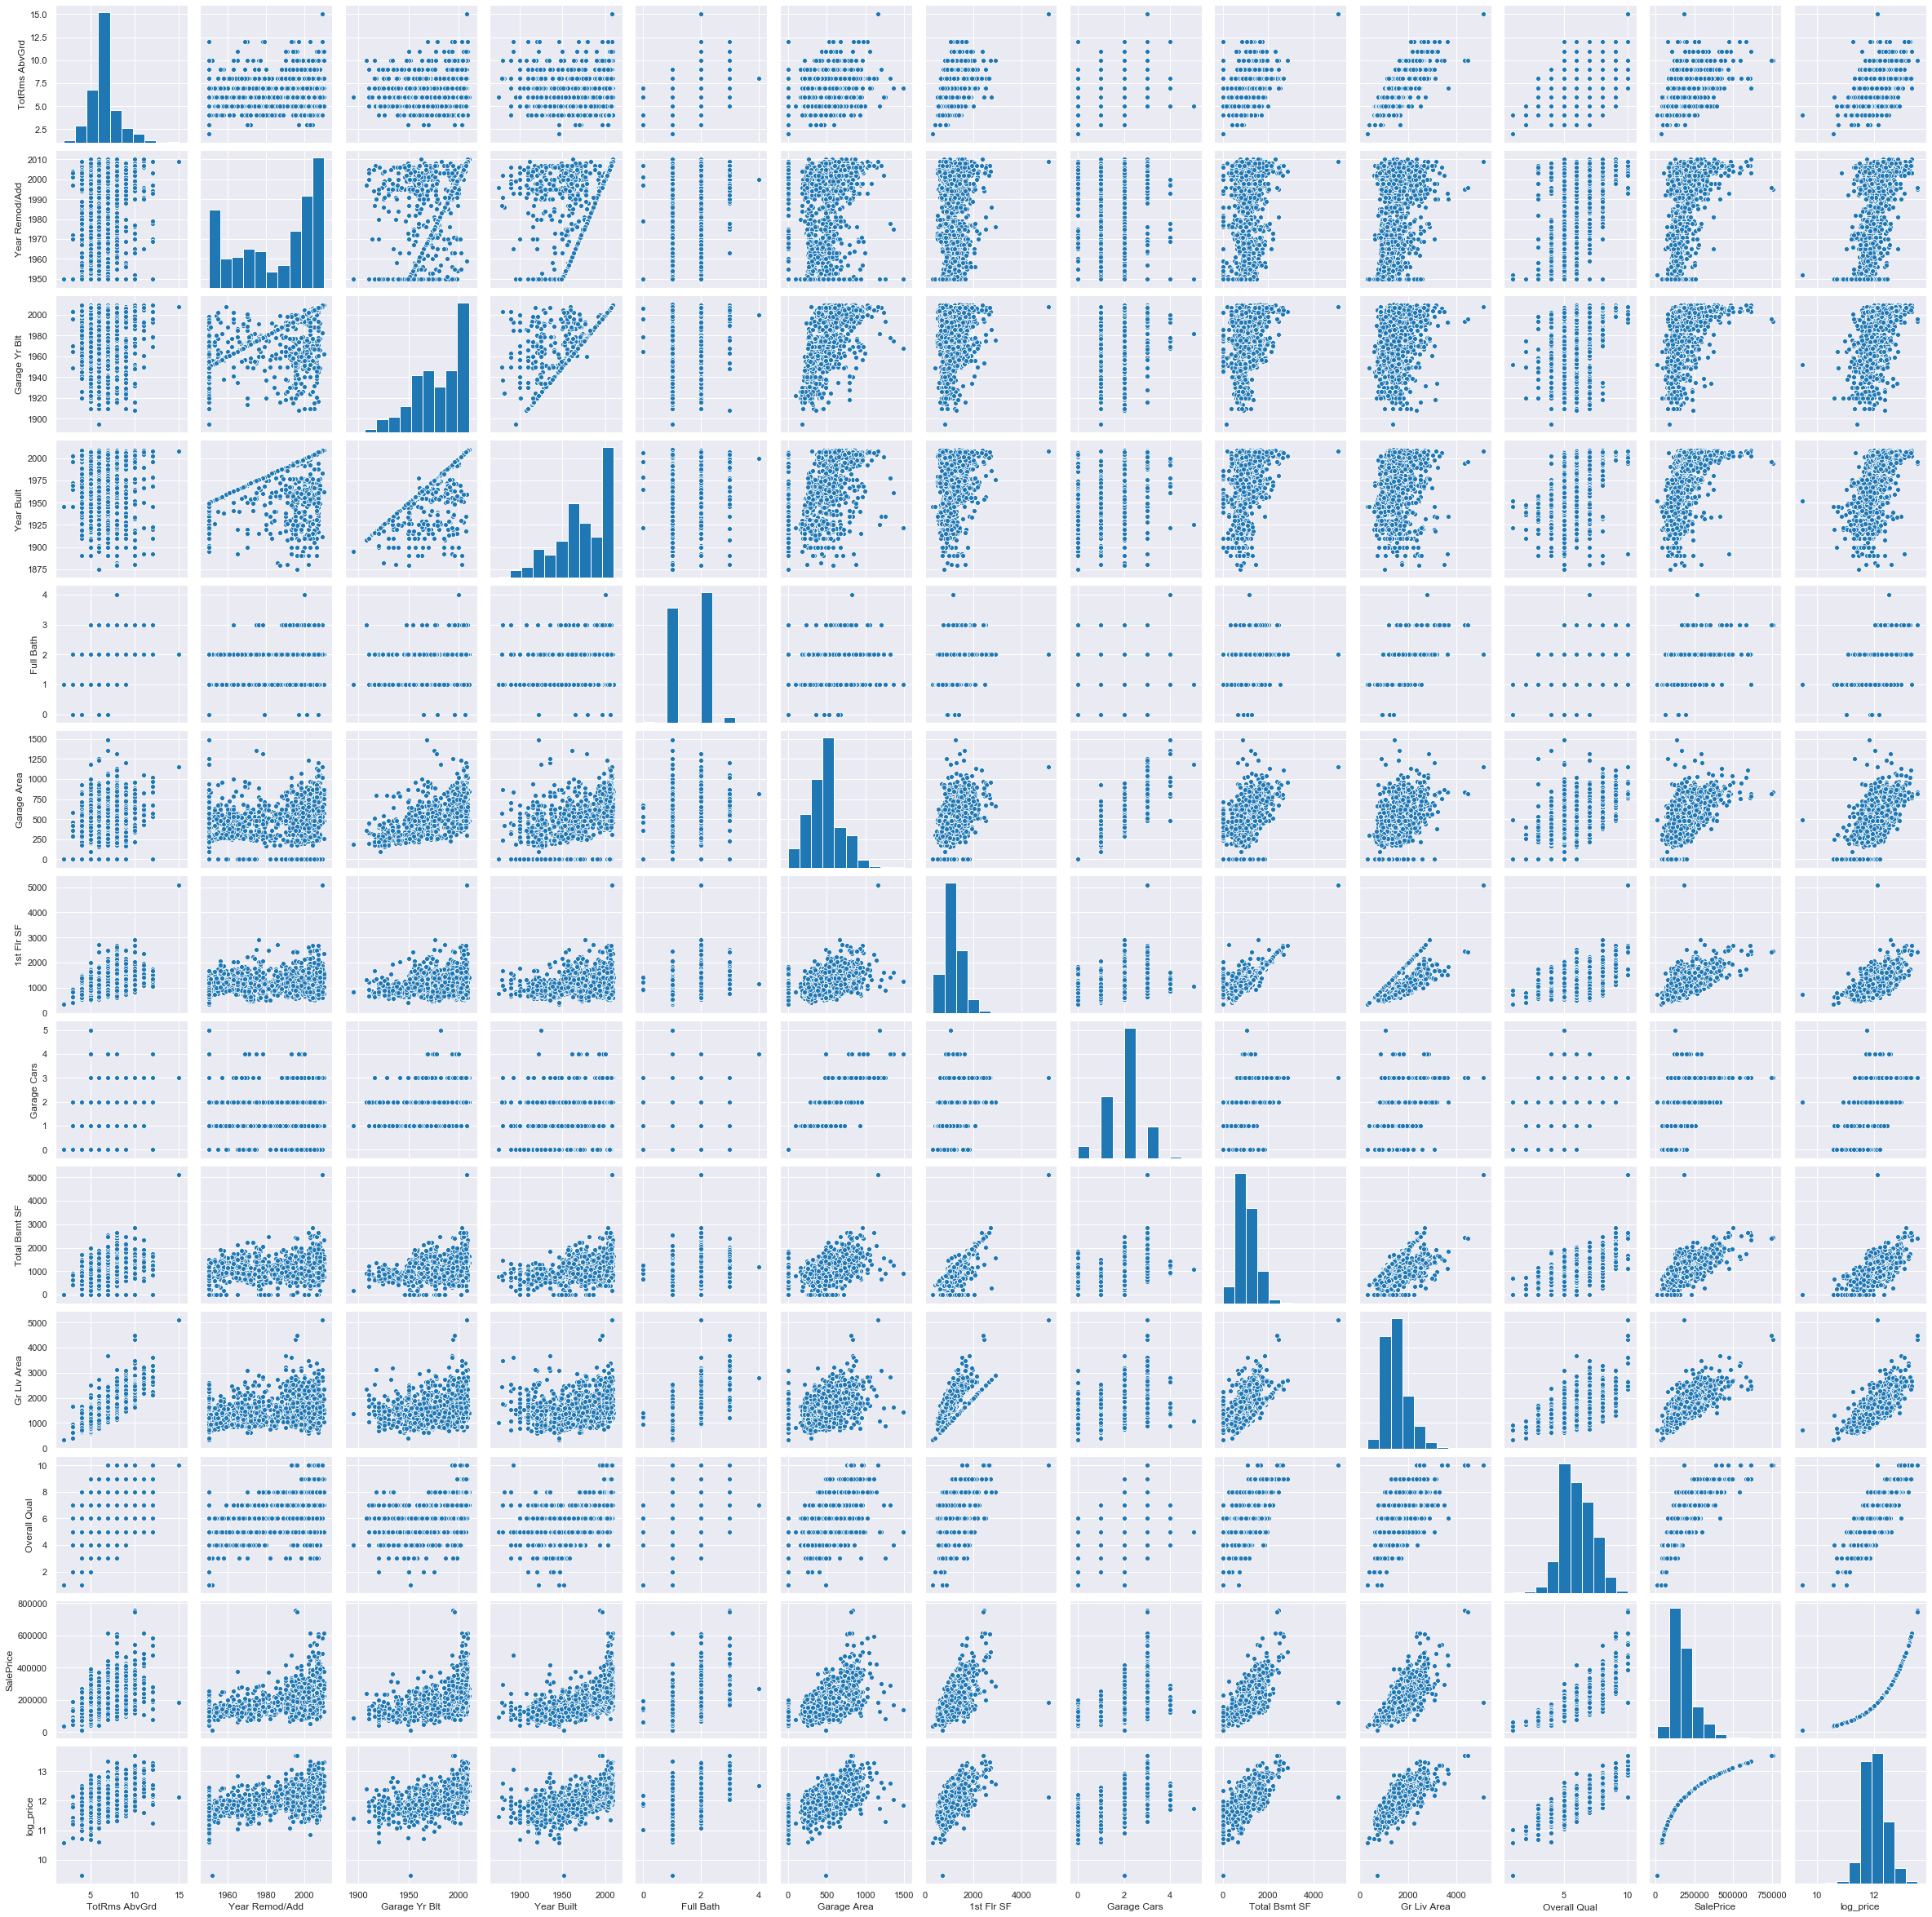
\includegraphics[width=0.8\textwidth]{scatter.png}
\centering
\caption{Distribution of numeric variables in housing data.}
\label{fig:scatter}
\end{figure}

\begin{figure}
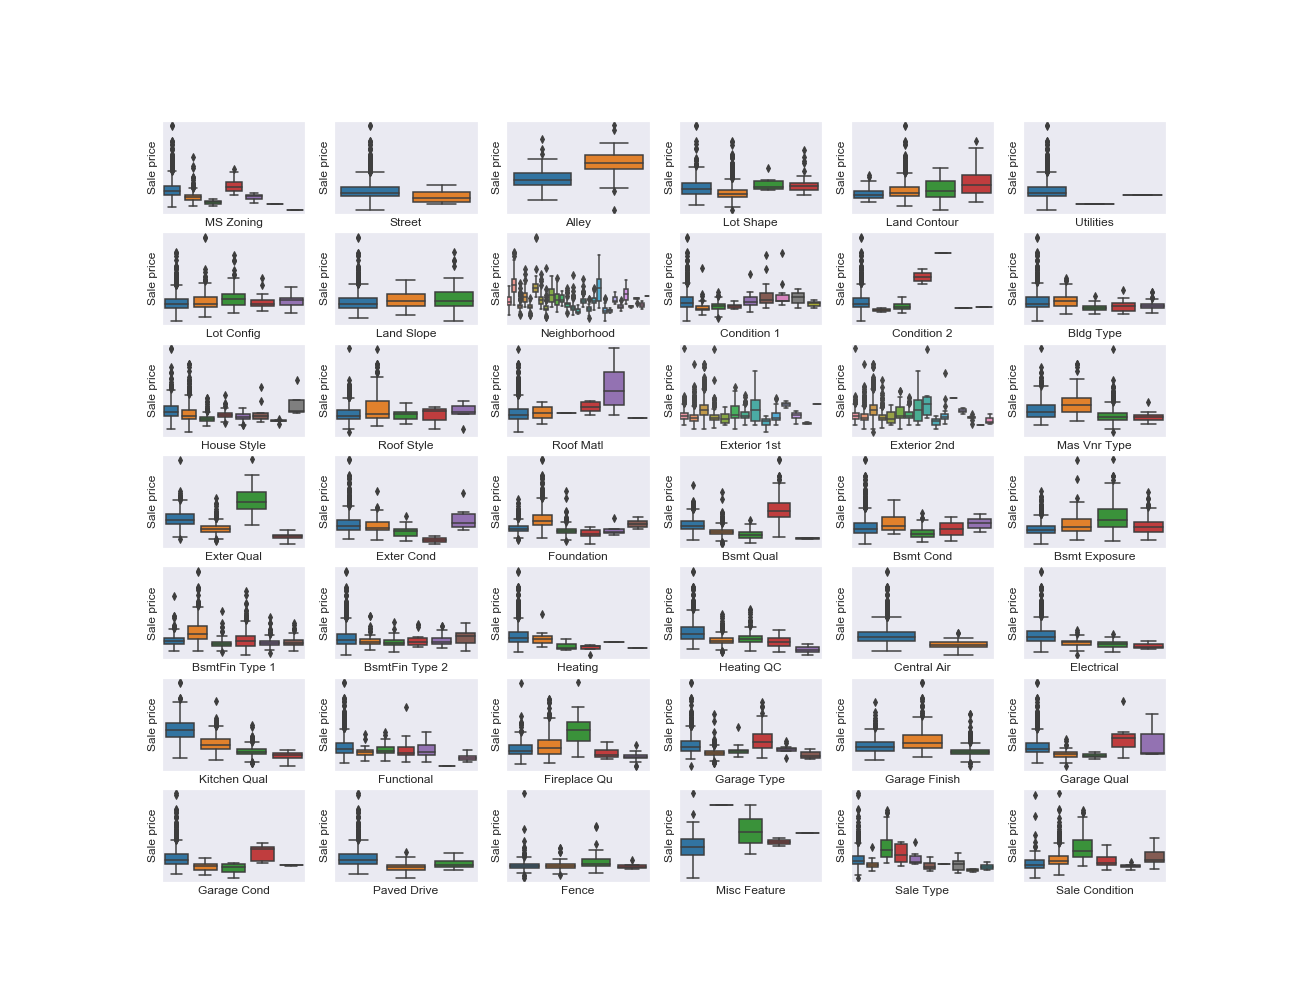
\includegraphics[width=0.8\textwidth]{boxplot.png}
\centering
\caption{Boxplots demonstrating distribution of sale price for houses with different categorical features in housing data.}
\label{fig:boxplots}
\end{figure}

%\showmatmethods


\bibliography{pinp}
\bibliographystyle{jss}



\end{document}

